%
% hauptkruemmungen.tex
%
% (c) 2017 Prof Dr Andreas Müller, Hochschule Rapperswil
%
\section{Hauptkrümmungen}
\rhead{Hauptkrümmungen}
In Abschnitt~\eqref{skript:kruemmung:richtungsabhaengigkeit} wurde gezeigt,
dass die Schnittkrümmungen $\kappa(e)$ in Abhängigkeit von der
Tangentenrichtung $e$ dank der Wahl eines speziellen Koordinatensystems
mit Hilfe der Matrix der zweiten Ableitung berechnet werden kann.
Wenn $e$ ein Einheitsvektor ist, dann haben wir gefunden, dass die
Schnittkrümmung
\[
\kappa(e)
=
2\biggl(
\frac{\partial^2 f}{\partial x^2}
e_1^2
+
2
\frac{\partial^2 f}{\partial x\partial y}e_1e_2
+
\frac{\partial^2 f}{\partial y^2}e_2^2
\biggr)
\]
ist.
In dieser Form ist nicht klar erkennbar, wie $\kappa(e)$ von $e$ abhängt.

Wir können $\kappa(e)$ aber auch in Vektorform schreiben.
Dazu schreiben wir die Matrix der zweiten Ableitungen als
\[
H
=
\begin{pmatrix}
\displaystyle\frac{\partial^2 f}{\partial x^2}&
\displaystyle\frac{\partial^2 f}{\partial x\partial y}\\
\displaystyle\frac{\partial^2 f}{\partial x\partial y}&
\displaystyle\frac{\partial^2 f}{\partial y^2}
\end{pmatrix},
\]
sie heisst die {\em Hessische Matrix}.
Damit kann die Krümmung als Matrizenprodukt geschrieben werden:
\[
\kappa(e)
=
\begin{pmatrix}e_1&e_2\end{pmatrix}
\begin{pmatrix}
\displaystyle\frac{\partial^2 f}{\partial x^2}&
\displaystyle\frac{\partial^2 f}{\partial x\partial y}\\
\displaystyle\frac{\partial^2 f}{\partial x\partial y}&
\displaystyle\frac{\partial^2 f}{\partial y^2}
\end{pmatrix}
\begin{pmatrix}e_1\\e_2\end{pmatrix}
=
e^tHe.
\]
Die Matrix $H$ ist offenbar symmetrisch.

\begin{figure}
\centering
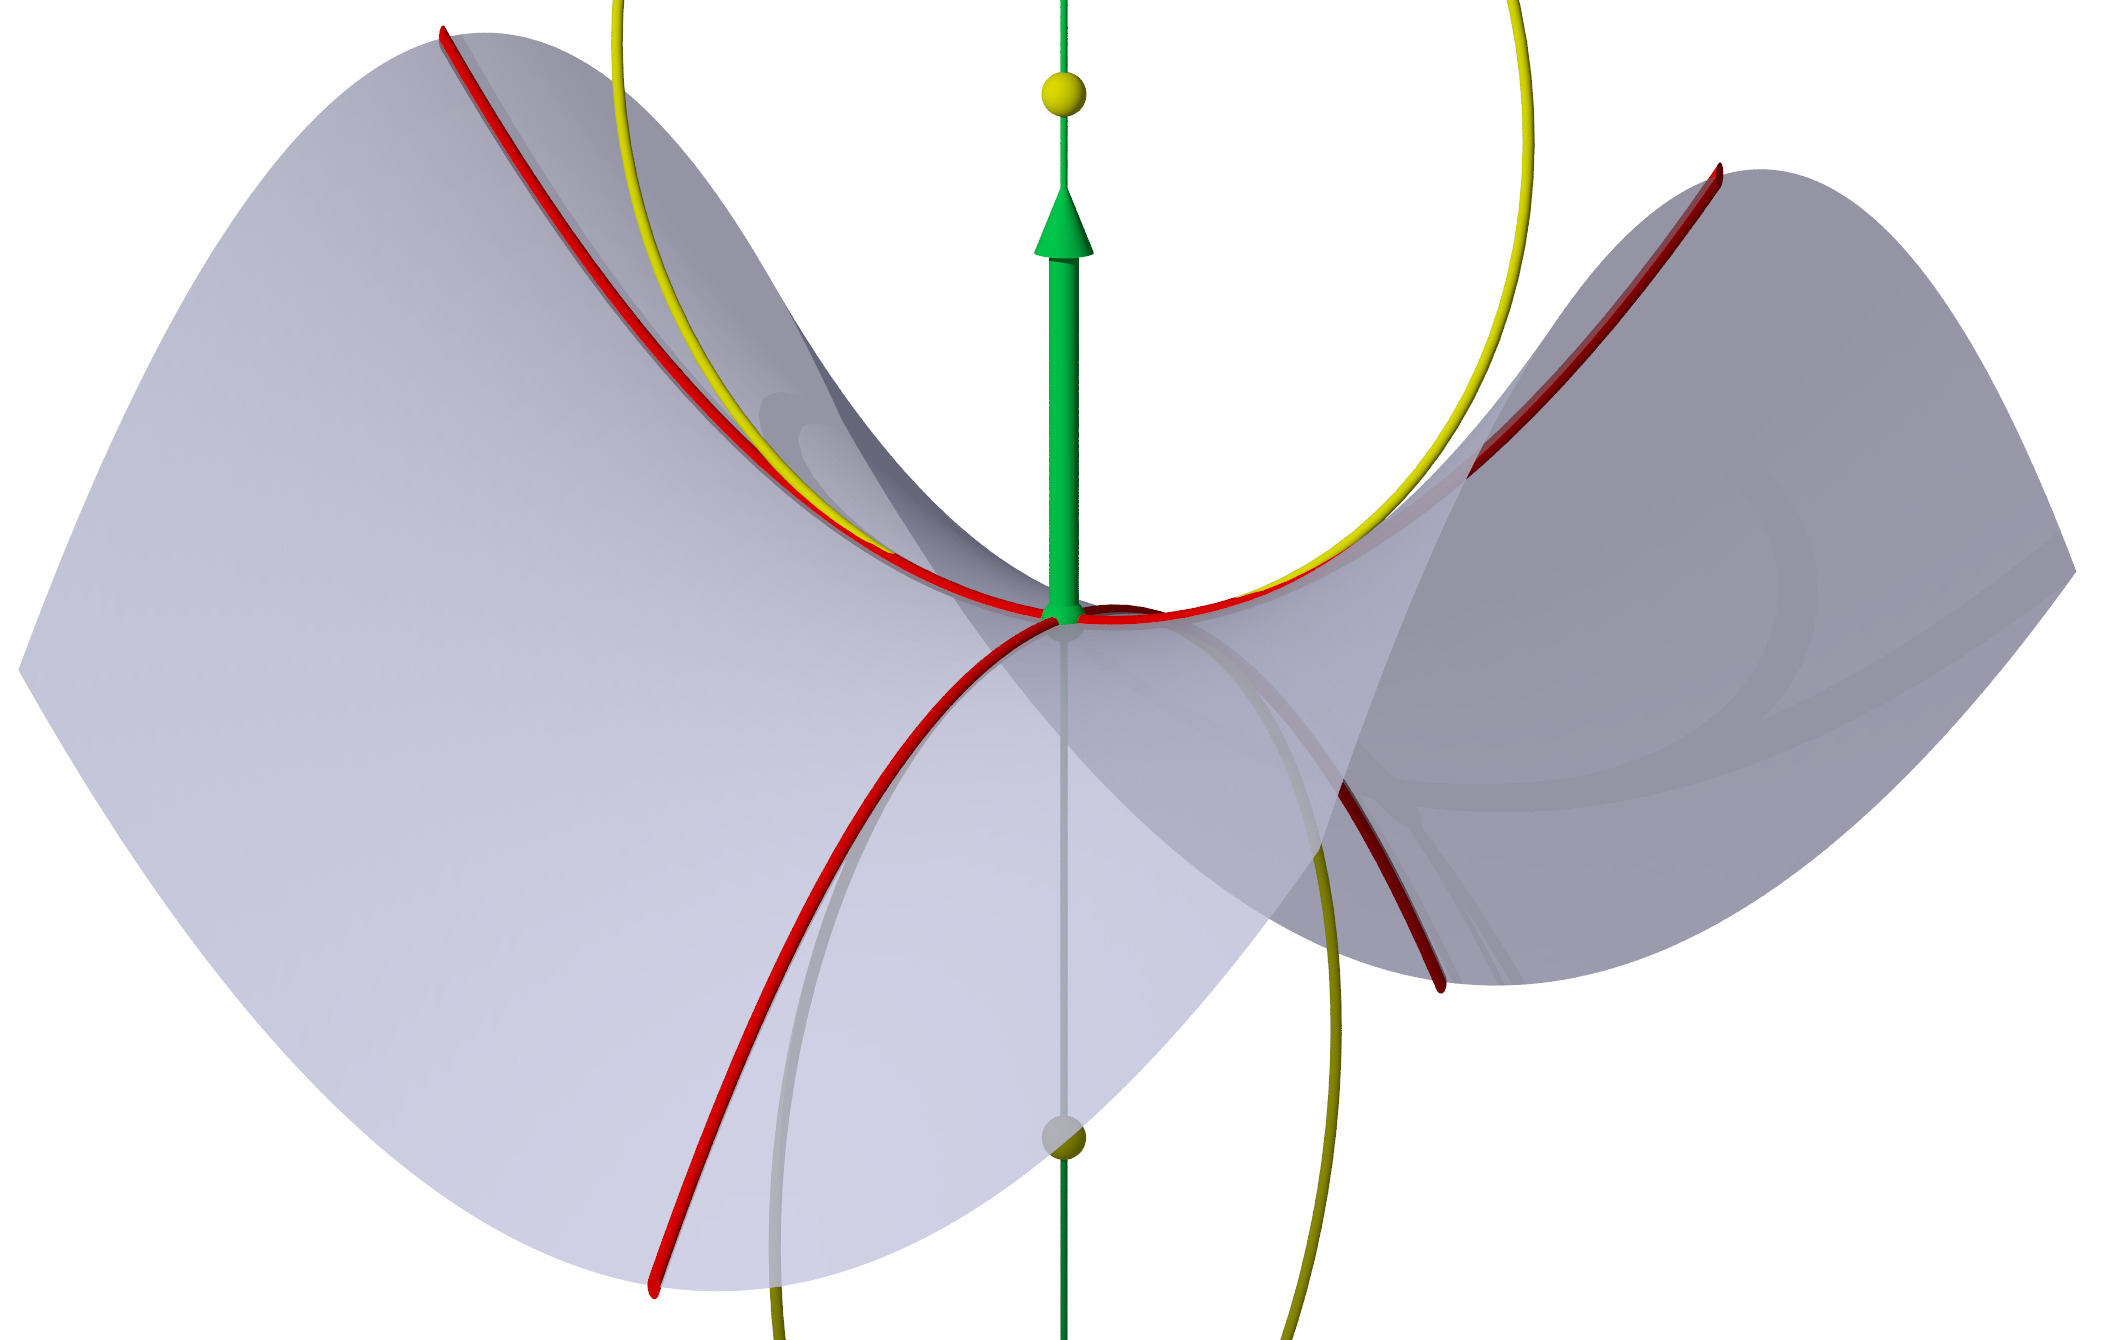
\includegraphics[width=\hsize]{chapters/3d/hauptkruemmungen.jpg}
\caption{Die Hauptkrümmungen einer Fläche sind die maximale und minimale
Schnittkrümmung in einem Punkte.
Die zugehörigen Krümmungsrichtungen heissen die Hauptkrümmungsrichtungen.
In diesem Beispiel haben die beiden Hauptkrümmungen verschiedenes Vorzeichen.
\label{skript:kurven:hauptkruemmungen}}
\end{figure}

In der linearen Algebra lernt man, dass sich jede symmetrische Matrix 
mit Hilfe einer Matrix in $\textrm{SO}(n)$ diagonalisieren lässt.
Im vorliegenden Fall gibt es eine Drehung der $x$-$y$-Ebene derart, dass
die Matrix $H$ Diagonalform bekommt.
Die Krümmung in Abhängigkeit vom Einheitsvektor $e$ ist daher
\[
\kappa(e)
=
2\lambda_1 e_1^2 + 2\lambda_2 e_2^2,
\]
wobei $\lambda_1$ und $\lambda_2$ die Eigenwerte von $H$ sind.
Für $e_1=\cos\alpha$ und $e_2=\sin\alpha$ bekommt man
\[
\kappa(\alpha)
=
2\lambda_1 \cos^2\alpha + 2\lambda_2 \sin^2\alpha.
\]
Diese Funktion nimmt ihr Maximum und Minimum auf den Achsen an,
die Eigenwerte sind also bis auf den Faktor $2$ die maximale und minimale
Schnittkrümmung.
Wir schreiben $\kappa_1=2\lambda_1$ und $\kappa_2=2\lambda_2$ für die
beiden zugehörigen Krümmungen.
\index{Hauptkrümmungen}
Diese heissen auch die Hauptkrümmungen, die Richtungen der Achsen heissen
die Hauptkrümmungsrichtung, und sie stehen senkrecht aufeinander, weil
\index{Hauptkrümmungsrichtung}
die Eigenvektoren einer symmetrischen Matrix zu verschiedenen Eigenvektoren
immer senkrecht aufeinander stehen.

\subsection{Invarianten}
Die hessische Matrix $H$ hat die Eigenwerte $\lambda_1$ und $\lambda_2$.
Diese sind für sich genommen nicht interessant.
Hingegen sind die Determinante und die Spur von $H$ Invarianten, die
unabhängig von der Richtung der Achsen in der $x$-$y$-Ebene sind.

\subsubsection{Determinante -- Gausskrümmung}
\index{Gausskrümmung}
\index{Krümmung!Gauss-}
Die Determinante von $H$ ist das Produkt der Eigenwerte, also
\[
\det H
=
\lambda_1\lambda_2
=
\frac14 (2\lambda_1) (2\lambda_2)
=
\frac14 \kappa_1\kappa_2.
\]
Das Produkt der Hauptkrümmungen $K=\kappa_1\kappa_2$
heisst {\em Gausskrümmung} der Fläche.
Es stellt sich heraus, dass die Gausskrümmung auch aus inneren Eigenschaften
der Fläche ermittelt werden kann
(Theorema Egregium von Gauss).
Wir werden in Kapitel~\ref{skript:chapter:kruemmung} 
mit der Riemannsschen Krümmung ein Konzept einer Krümmung eines Raumes
definieren, welches für Flächen im Wesentlichen mit der Gausskrümmung
übereinstimmt.

\subsubsection{Spur -- mittlere Krümmung}
\index{mittlere Krümmung}
\index{Krümmung!mittlere}
Die Spur von $H$ ist eine weitere Invariante der Matrix.
Wir nennen
\[
\operatorname{Spur} H
=
\lambda_1+\lambda_2
=
\frac12(2\lambda_1+2\lambda_2)
=
\frac12(\kappa_1+\kappa_2)
\]
die {\em mittlere Krümmung}.
Die mittlere Krümmung ist wichtig zur Charakterisierung von Minimalflächen.









